\documentclass[border=8pt]{standalone}
\usepackage{tikz}
\usetikzlibrary{arrows.meta,positioning,calc}
\begin{document}
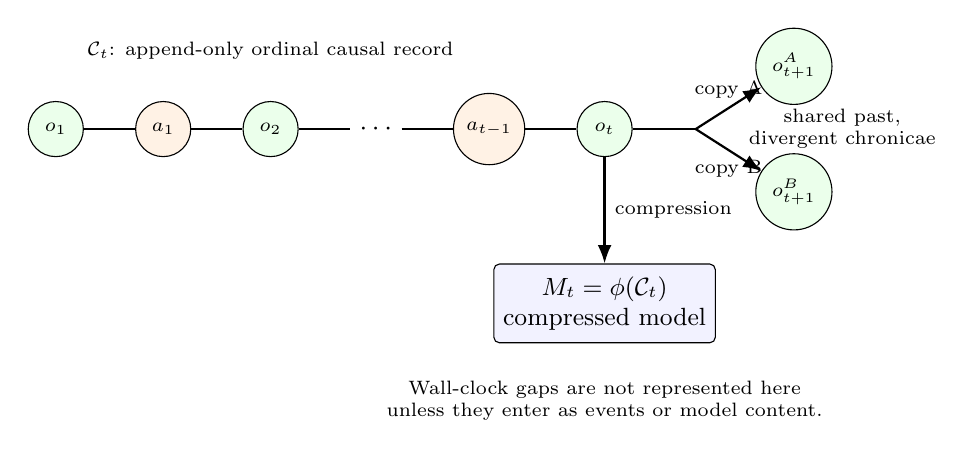
\begin{tikzpicture}[
  event/.style={circle, draw, minimum size=7mm, font=\scriptsize, fill=white},
  obs/.style={event, fill=green!8},
  act/.style={event, fill=orange!10},
  model/.style={draw, rounded corners=2pt, align=center, minimum width=2.6cm, minimum height=1.0cm, font=\small, fill=blue!5},
  arr/.style={-Latex, thick},
  hist/.style={thick},
  note/.style={align=center, font=\scriptsize}
]

\node[obs] (o1) {$o_1$};
\node[act, right=0.65cm of o1] (a1) {$a_1$};
\node[obs, right=0.65cm of a1] (o2) {$o_2$};
\node[right=0.65cm of o2] (dots) {$\cdots$};
\node[act, right=0.65cm of dots] (atm1) {$a_{t-1}$};
\node[obs, right=0.65cm of atm1] (ot) {$o_t$};

\draw[hist] (o1) -- (a1) -- (o2) -- (dots) -- (atm1) -- (ot);
\node[note, above=0.4cm of o2] {$\mathcal C_t$: append-only ordinal causal record};

\node[model, below=1.35cm of ot] (M) {$M_t=\phi(\mathcal C_t)$\\compressed model};
\draw[arr] (ot) -- node[right, note] {compression} (M);

\coordinate (fork) at ($(ot.east)+(0.8,0)$);
\draw[hist] (ot) -- (fork);
\node[obs, above right=0.45cm and 0.9cm of fork] (oA) {$o_{t+1}^A$};
\node[obs, below right=0.45cm and 0.9cm of fork] (oB) {$o_{t+1}^B$};
\draw[arr] (fork) -- node[above, note] {copy A} (oA);
\draw[arr] (fork) -- node[below, note] {copy B} (oB);
\node[note, right=0.55cm of fork] {shared past,\\divergent chronicae};

\node[note, below=0.35cm of M] {Wall-clock gaps are not represented here\\unless they enter as events or model content.};

\end{tikzpicture}
\end{document}
